\documentclass{article}
\usepackage[margin=2.5cm]{geometry}
\usepackage{enumerate}
\usepackage{fancyhdr}
\usepackage{graphicx}
\usepackage{amsmath}
\usepackage{tikz}
\usepackage{csvsimple}
\usepackage{pgfplots}

\pagestyle{fancy}
\fancyhead{}
\fancyfoot{}
\rfoot{\thepage}

\usepackage{float}
\usepackage{listings, color, times, textcomp, float, hyperref, subcaption}
\definecolor{mygreen}{RGB}{28,172,0} % color values Red, Green, Blue
\definecolor{mylilas}{RGB}{170,55,241}
\lstset{language=Matlab, basicstyle=\scriptsize\ttfamily,breaklines=true,frame=single,morekeywords={matlab2tikz},
keywordstyle=\color{blue}, morekeywords=[2]{1}, keywordstyle=[2]{\color{black}}, identifierstyle=\color{black},
stringstyle=\color{mylilas}, commentstyle=\color{mygreen}, showstringspaces=false, numbers=left,
numberstyle={\tiny \color{black}}, numbersep=9pt, emph=[1]{for,end,break},emphstyle=[1]\color{red},
literate={~} {\texttildelow}{1}}

\title{MATH 3610 - Project \#1}
\author{Paul Chesnais (pmc85), Christopher Silvia (cps232), Ryan Vogan (rcv39)}
\date{\today}

\newcommand{\exo}[1]{\section*{Exercise #1}}
\newcommand{\prob}[1]{\section*{Problem #1}}
\newcommand{\quest}[1]{\section*{Question #1}}
\newcommand{\e}{&=}
\newcommand{\p}[1]{\times 10^{#1}}
\renewcommand{\headrulewidth}{0pt}
\renewcommand{\footrulewidth}{0.5pt}

\DeclareMathOperator\erf{erf}

\begin{document}
\maketitle
\thispagestyle{fancy}

\section{Decision Variables}

The client has proposed two strategies:

\begin{enumerate}
\item Focus vaccination efforts on the ``most connected''.
\item Focus vaccination efforts on the most frail or susceptible.
\end{enumerate}

In our models, we want to express our choice of policy as a ``decision variable''.
Since we will be recieving 4000 vaccinations a month, our policy recommendation
	will be how to distribute those 4000 vaccinations.
If we identify $n$ categories of Ithacans, each month we will provide
	recommendations on which fraction of the 4000 vaccines to give to
	each category of Ithacans.

We should note that each model won't necessarily divide the population into the
	same number of categories.
Each one will provide a different recommendation for the health officials.

\section{Evaluating Models}

Once we chose parameters for our model, we will run it and show its predictions.
We expect that models should at least model the total number of sick
	individuals.
The model might also keep track of how many individuals die.
We have thought of three different ways of evaluating our model:

\begin{enumerate}
\item Total Deaths
\item Total Person-Days Spent Sick
\item Time Until Disease is Eradicated
\end{enumerate}

Note that the models may only provide predictions for some of these criteria.

\section{Simple Continuous Model}

First, we propose a deterministic model which doesn't divide the population
	into sections at all.
This model will help give us an idea of what the effect of dividing
	the population into sections will be.
In addition, it can give us an idea of how vaccination affects the spread of
	disease within a population.

\subsection{Disease Spread with No Vaccine}

We include this derivation of the logistic model for disease spread
	to compare with our derivation of the modified logistic model
	for disease spread and vaccination.

Suppose there are two groups of people, with $I$ representing the number of
	infected people, and $S$ represnting the number of people seceptible for the
	disease.
Suppose the probability of a single healthy person becoming sick is proportional
	only to the total number of sick people.
Since there are $S$ healthy people, the expected number of healthy people
	who become sick should be proportional to $S I$.
This model does not take into account recovery from sickness.
If we introduce a parameter $r$, we can express this relationship as a system
	of differential equations:

\begin{align*}
\frac{dS}{dt} & = - r S I \\
\frac{dI}{dt} & = r S I \\
\end{align*}

Notice that the total number of people, $S + I$, is conserved, i.e.,

\[ \frac{d}{dt} \left( S + I \right) = \frac{dS}{dt} + \frac{dI}{dt}
	= r S I - r S I = 0 \]

If we introduce another parameter, $K$, to represent the total population,
	such that $S + I = K$ for all time, then the differential equations
	can be decoupled:

\begin{align*}
\frac{dS}{dt} & = - r S (K - S) \\
\frac{dI}{dt} & = r (K - I) I \\
\end{align*}

The two differential equations shown here are now two independant, uncoupled
	differential equations which we can solve seperately.

\subsubsection{Nondimensionalizing the Model}

It would be helpful to make all of the constants dimensionless parameters.
This will give us insight into the different scales that the model works at.

To turn $I$ into a dimensionless parameter, we can divide by $K$.

\begin{align*}
\frac{d\left(\frac{I}{K}\right)}{dt}
	& = \left( r K \right) \left( \frac{I}{K} \right) \left( 1 - \frac{I}{K} \right)\\
\frac{d\widetilde{I}}{dt}
	& = \widetilde{r} \widetilde{I} \left( 1 - \widetilde{I} \right)
\end{align*}

This shows that the dynamics of $I$ do not depend on its size.
For each value of the dimensionless constant $\widetilde{r}$,
	we determine the behavior from it.

\subsection{Diease Spread with Vaccine}

Suppose we introduce a third group, $V$ for vaccinate, representing people who are
	immune from the diesease.
Right now, the only way to become immune is through vaccination,
	but we may add recovery in subsequent models.
Suppose we randomly vaccinate members of the healthy population,
	a constant number each time step.
This introduces a third parameter, $r_v$, the rate of vaccinations.
The vaccinated population isn't seceptible to the disease.
This process is modeled by the following system of diffential equations:

\begin{align*}
\frac{dI}{dt} & = r S I \\
\frac{dS}{dt} & = - r S I - r_v \\
\frac{dV}{dt} & = r_v
\end{align*}

This model is accurate only if all three of the populations remain
	positive.
This is important to remember.
The number of healthy people will always be decreasing, so once
	the number of healthy people hits zero, we stop the model.
The sick people stay sick, and the vaccinated people stay vaccinated.

The number of vaccinated people as a function of time is:

\[ V(t) = r_v t \]

Again, we find the conserved quantity $\left( S + I + V \right)$ and
	name it $K$.
For the model to be valid, we need $S = K - I - V \geq 0$.
Therefore, the model is valid as long as:

\[ K \geq I + r_v t \]

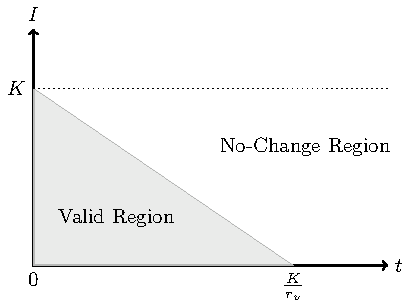
\includegraphics[width=0.5\textwidth]{figures/admissible-region.pdf}

In the above figure, once $I(t)$ hits the diagonal line,
	it stays horizontal and keeps its value.

We have now made these differential equations independant,
	within the model's zone of validity:

\begin{align*}
\frac{dI}{dt} & = r I \left( K - I - r_v t \right)\\
\frac{dS}{dt} & = - r S \left( K - S - r_v t \right) - r_v \\
\frac{dV}{dt} & = r_v t
\end{align*}

We present a solution for $I(t)$ \cite{walph}:

\begin{align}
I(t) & =
	\frac{e^{ r t (K - \frac{ r_v t}{2})}}
	{\frac{1}{S(0)} + \sqrt{\frac{\pi r}{2 r_v}}
		e^{\frac12 \left( \frac{r}{r_v} \right) K^2}
		\left(\erf\left(  \sqrt{\frac{r}{2 r_v}} (r_v t - K ) \right)
			- \erf\left( - \sqrt{\frac{r}{2 r_v}} K \right) \right)}
\end{align}

From the above expression for the boundary of the valid region,
	we get the following implicit expression for $t_f, I(t_f)$

\begin{align}
I(t_f) =
	\frac{e^{ r t_f (K - \frac{ r_v t_f }{2})}}
	{\frac{1}{S(0)} + \sqrt{\frac{\pi r}{2 r_v}}
		e^{\frac12 \left( \frac{r}{r_v} \right) K^2}
		\left(\erf\left(  \sqrt{\frac{r}{2 r_v}} (r_v t_f - K ) \right)
			- \erf\left( - \sqrt{\frac{r}{2 r_v}} K \right) \right)}
	& = K - r_v t_f
\end{align}

Here is a family of values of $I(t)$.
The total population and the rate of distributing vaccines are
	held constant, while each curve corresponds to a different
	value of the growth rate constant.
Each curve starts with an initial condition at 5 percent of the
	population, and the growth rate determines how many people
	overall are infected.

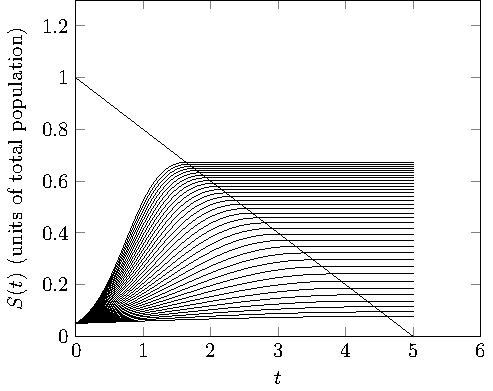
\includegraphics[width=0.5\textwidth]{figures/vaccination-model-curves-varying-s.pdf}


\subsection{Pareto Optimizing Between Two Independent Populations}

The model above modeled how one population responds to a combination
	of disease spreading and vaccines.
The model depends on $K$, the total population, $I(0)$, the initial
	number of sick people, $r$, the rate of infection growth,
	and $r_v$, the vaccination rate.
Of these parameters, in a real world setting, we can expect to know $K$
	very precicely from census data, approximate $I(0)$ as small,
	have very little idea about $r$, and control $r_v$.

I want to extend this problem to two independant populations.
Each population will get different sets of constants,
	$K_1$ and $K_2$, $I_1(0)$ and $I_2(0)$, $r_1$ and $r_2$.
The goal will be to figure out how to optimally allocate the
	vaccines between the two populations.
The decision variable, $d$, will be the fraction of the total vaccination
	rate I allocate to each population.
Population 1 will be vaccinated at a rate $d r_v$, while population
	2 will be vaccinated at a rate $(1 - d) r_v$.
In this model, I try to minimize the final number of sick people in
	each population.
This will give me a pareto front.

The following collection of pareto fronts comes from keeping the disease
	growth rate the same for both, and varying its magnitude.

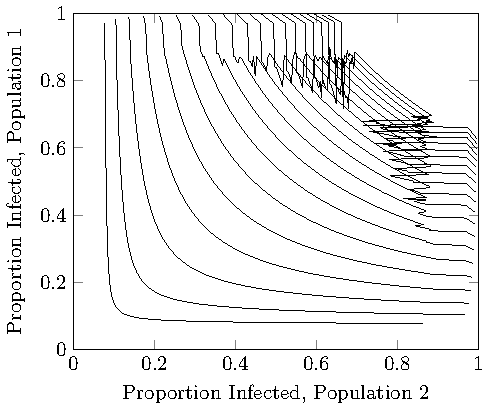
\includegraphics[width=0.5\textwidth]{figures/vaccination-model-same-r-pareto-curves.pdf}

This collection of pareto fronts comes from keeping the growth
	rate for population 2 the same, and varying the growth
	rate of population 1.

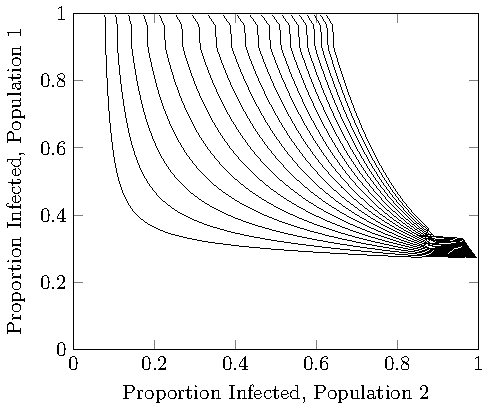
\includegraphics[width=0.5\textwidth]{figures/vaccination-model-different-r-pareto-curves.pdf}

\subsection{Improved Model}

In the preceding model, once people became infected, they stayed
	infected for the duration of the run.
The following model adds a parameter, the ``curing rate'' $\gamma$,
	which represents the rate at which individuals in the sick population
	recover (and join the removed population).
This model is the SIR model, and has standard parameters:

\begin{align*}
\frac{dI}{dt} & = \frac{ \beta S I}{N} - \gamma I\\
\frac{dS}{dt} & = -\frac{\beta S I}{N} - r_v \\
\frac{dR}{dt} & = r_v + \gamma I
\end{align*}

We can use this model for pareto optimization.
Cornell's population is about 21,000 \cite{cornellpop},
	while ithaca's population is about 30,000 \cite{census}.
Given a rate of vaccine distribution, by integrating the equations
	we can determine how many total infections there are.
If we had 4000 vaccinations to distribute, we can make a pareto
	curve by plotting the set of points corresponding to different
	relative distributions of the vaccinations.

If one of the populations vaccinates all of its seceptible individuals
	before the other, we need to decide what to do with the vaccines
	that it is not consuming.
If we choose not to redistribute them, the pareto curve looks like this:

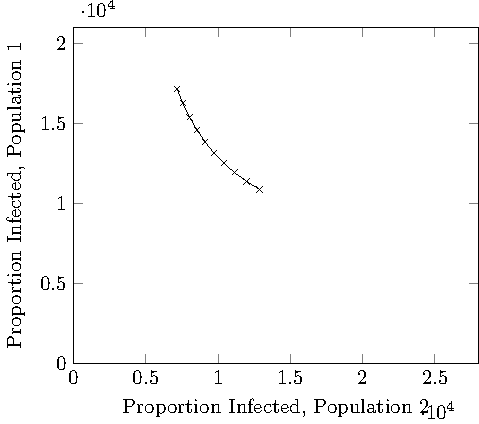
\includegraphics[width=0.5\textwidth]{figures/sir-pareto.pdf}

If we choose to redistribute them, for $\beta = 6$ and $\gamma = 4$,
	the curve looks like this:

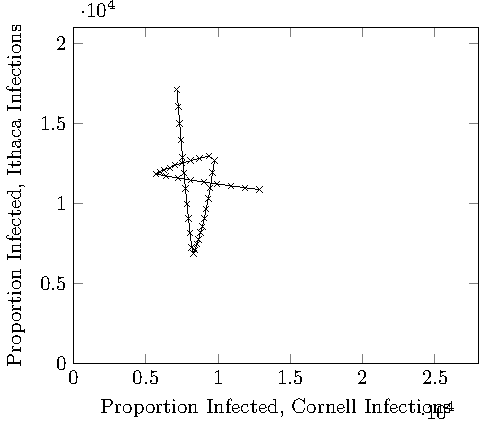
\includegraphics[width=0.5\textwidth]{figures/sir-pareto-top.pdf}

And the pareto curve looks like:

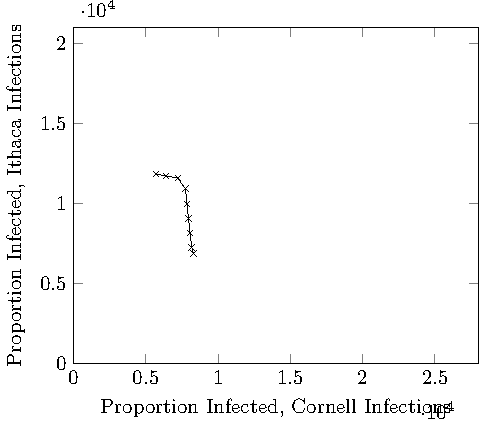
\includegraphics[width=0.5\textwidth]{figures/sir-pareto-top-pareto.pdf}

We conclude that making sure that all of the vaccines are allocated is very
	important for any vaccine model, noting the difference.
The pareto-optimal points are when 71-84\% of the vaccine goes to the
	cornellians and 29-16\% goes to the ithacans,
	and when 15-20\% of the vaccine goes to the cornellians
	and 80-85\% of the vaccine goes to the ithacans.

\subsection{Disease Spread between Coupled Populations}

Consider three populations, with two connected only by an intermediate
	one.


\begin{align*}
\frac{d\widetilde{I}_1}{dt} & = \left( \left( r_{11} K_1 \right) \widetilde{I}_1
			+ \left( r_{12} K_2 \right)  \widetilde{I}_2 \right)
		\left( 1 - \widetilde{I}_1 - \left( \frac{\alpha_1}{K_1} \right) t \right)\\
\frac{d\widetilde{I}_2}{dt} & = \left( \left( r_{22} K_2 \right) \widetilde{I}_2
			+ \left( r_{21} K_1 \right)  \widetilde{I}_1
			+ \left( r_{23} K_3 \right) \widetilde{I}_3 \right)
		\left( 1 - \widetilde{I}_2 - \left( \frac{\alpha_2}{K_2} \right) t \right)\\
\frac{d\widetilde{I}_3}{dt} & = \left( \left( r_{33} K_3 \right) \widetilde{I}_3
			+ \left( r_{32} K_2 \right)  \widetilde{I}_2 \right)
		\left( 1 - \widetilde{I}_3 - \left( \frac{\alpha_3}{K_3} \right) t \right)
\end{align*}

If the second population is relatively small, then we might be able to
	decrease the total number of infections by focusing our entire efforts
	on the smallest population to cut the link between the two populations.
We then treat the vaccination problem as a pareto optimization problem, to distribute
	the vaccines amongst the two populations.
However this may not be better than splitting the vaccinations between the two.

\section{Stochastic Model}
\subsection{A naive model}
\par At first, we made a simple, arbitrary stochastic model just to get a rough idea of how the disease would spread. Over the course of 5 months, we would look at the spread of the disease given certain conditions. Every citizen fell into an age category, according to demographic figures from \emph{areaConnect} \cite{areconnect}. Then, to model the spread, we associated arbitrary recovery rates, complication rates and number of people talked to per month to each age group, giving us the following table:
\begin{figure}[h!]
\centering
\begin{tabular}{c|c|c|c|c}
Age group & Heal rate & Complication chance & Connectivity & Population percentage\\ \hline
Kids & 0.5 & 0.2 & 20 & 10\%\\
Teens & 0.4 & 0.1 & 30 & 40\%\\
Adults & 0.3 & 0.3 & 25 & 40\%\\
Seniors & 0.2 & 0.7 & 10 & 10\%
\end{tabular}
\caption{Initial citizen attributes}
\end{figure}

\par The Heal rate and Complication chance columns represent the odds of a given citizen to recover from the disease in a month. The Connectivity column represents the number of people each sick citizen has a chance to infect, uniformly sampled from the entire population. We would then infect 500 people initially, and let the simulation run its course. In this particular example, we vaccinate randomly. We also assume that a person who has been sick cannot be sick again, and that when complications arise in a given patient, they are taken to the hospital and do not keep infecting the rest of the population. Here's how the spread of disease looks:
\begin{figure}[h!]
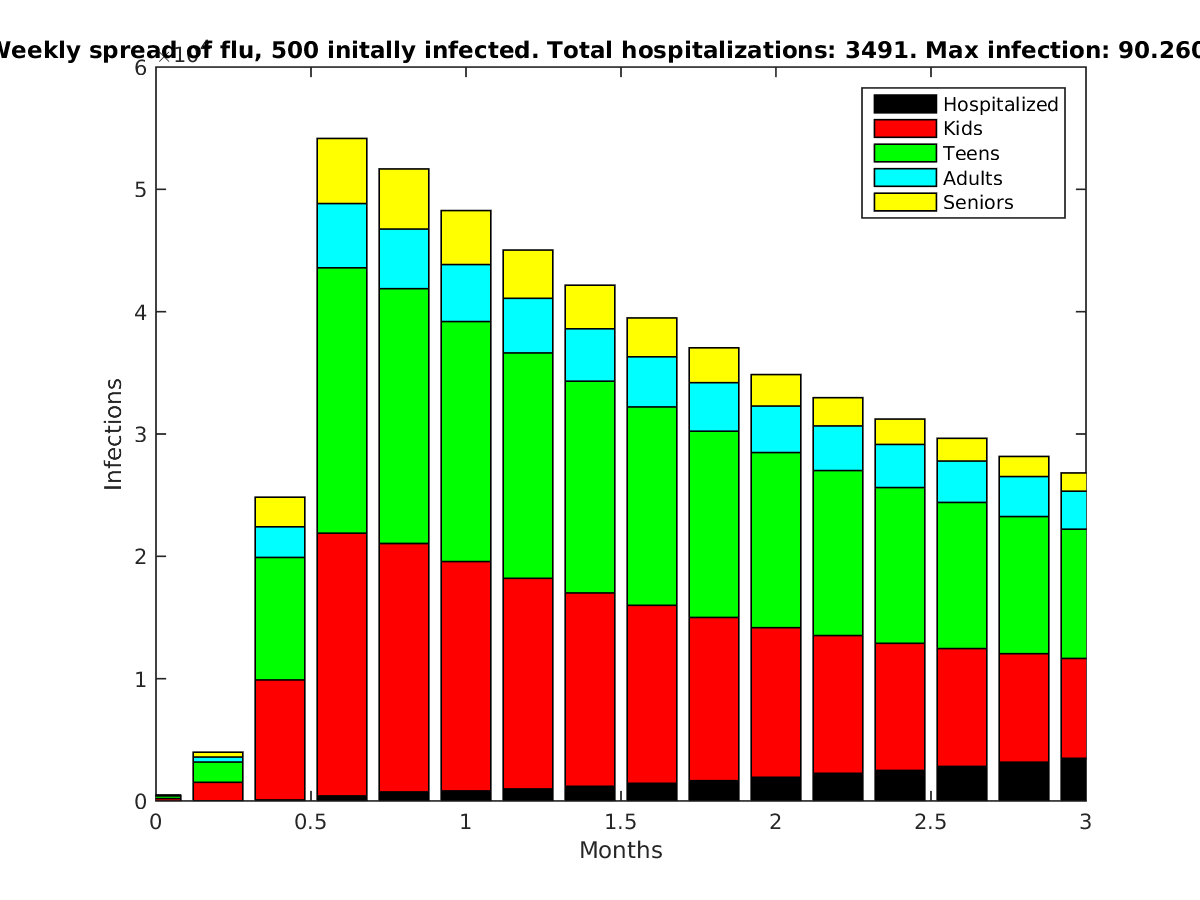
\includegraphics[width=\textwidth]{figures/Naive-model.png}
\caption{Initial model predictions}
\end{figure}
The parts of each bars represent the respective number of citizens in a given age group that are sick. The black bars on the bottom represent how many people have been hospitalized so far.
\par Unfortunately, research and according to sources from the CIC \cite{CIC-stats} \cite{CIC-qa} exposed many flaws in this model. Mostly the fact that the odds of a given citizen staying sick for more than a month are extremely low, unlike in this model where they are actually quite high. In fact, every age range stays sick for just about the same amount of time, with seniors sick for 2 weeks. The CIC data also exposed something very interesting, which is that seniors are not the ones in the most danger from the flu, kids smaller than the age of 5 are. This gave us reason to use a model that looks at the spread of the disease on a weekly basis.

\subsection{A more justified approach}
\par As mentioned in earlier, the CIC data gave us a lot to think about in terms of refining this model. First of all, we looked at the effects of the population of children in Ithaca, where children are citizens younger than 5 years of age. Since their risks of complications are so much higher, a good idea would be to immediately vaccinate all of them to avoid a devastating death toll. Fortunately, according to \emph{areaConnect}, there are less than 2,000 children in Ithaca, meaning that they can all be vaccinated as soon as the shipment of vaccines arrives. This also means that we can cut out an entire segment of the population, and generalize citizens younger than 25 years of age to a single slice. As a slight additional adaptation, we also make it such that any given citizen is more likely to talk to people from their age slice.
\par Secondly, we obtained more concrete data on how long citizens stay sick, and the likelihood of complications. The data we found was given in terms of weeks, so we changed the model to compute the spread on a weekly basis. For averaging and rounding, we assumed that there are 4 weeks in a month, and that all citizens, regardless of age, have a 90\% of healing every week. According to the CIC, a patient infected by the H1N1 virus is only contagious when showing symptoms. Therefore a citizen only infects other citizens when they are sick. Given what we know about the H1N1 virus and how contagious it is, we take 80\% to be the chance that a sick citizen infects a healthy one, with the 20\% accounting for sanitary precautions like hand sanitizer (assuming people don't have ``Swine flu Parties'' \cite{CIC-qa}).
\par With this in mind, we adapted the model such that each age group had the attributes listed in Figure~\ref{fig:justified-values}:

\begin{figure}[h!]
	\centering
	\begin{tabular}{c|c|c|c|c}
		Age group & Heal rate & Complication chance & Connectivity & Population percentage\\ \hline
		Junior & 0.9 & 0.05 & 25 & 60\%\\
		Adults & 0.9 & 0.2 & 15 & 30\%\\
		Seniors & 0.9 & 0.75 & 5 & 10\%
	\end{tabular}
	\caption{More justified attributes for age groups}
	\label{fig:justified-values}
\end{figure}

Here are a handful of runs for different vaccination strategies:
\begin{figure}[h!]
	\centering
	\begin{subfigure}[b]{0.5\textwidth}
		\centering
		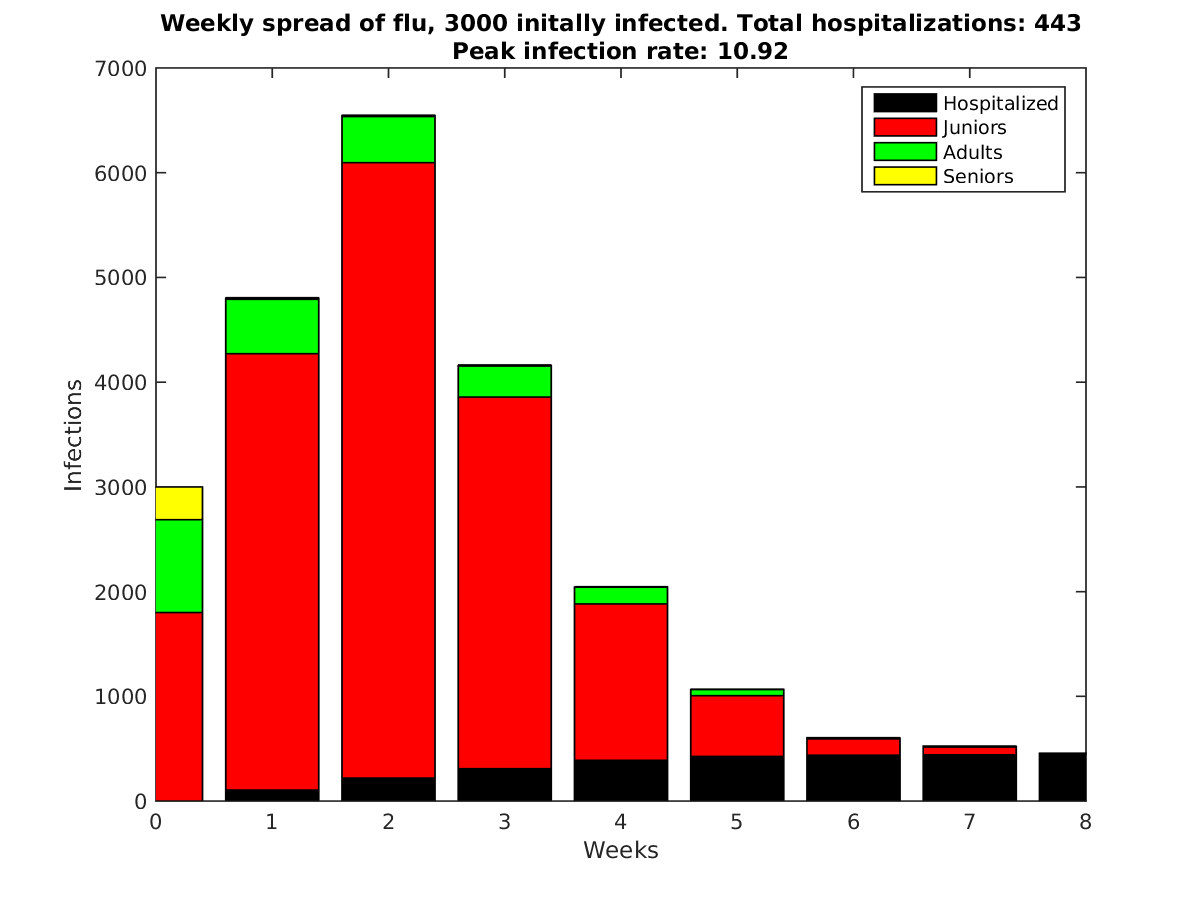
\includegraphics[width=\textwidth]{figures/Weekly-novax.png}
		\caption{No vaccination policy}
	\end{subfigure}~
	\begin{subfigure}[b]{0.5\textwidth}
		\centering
		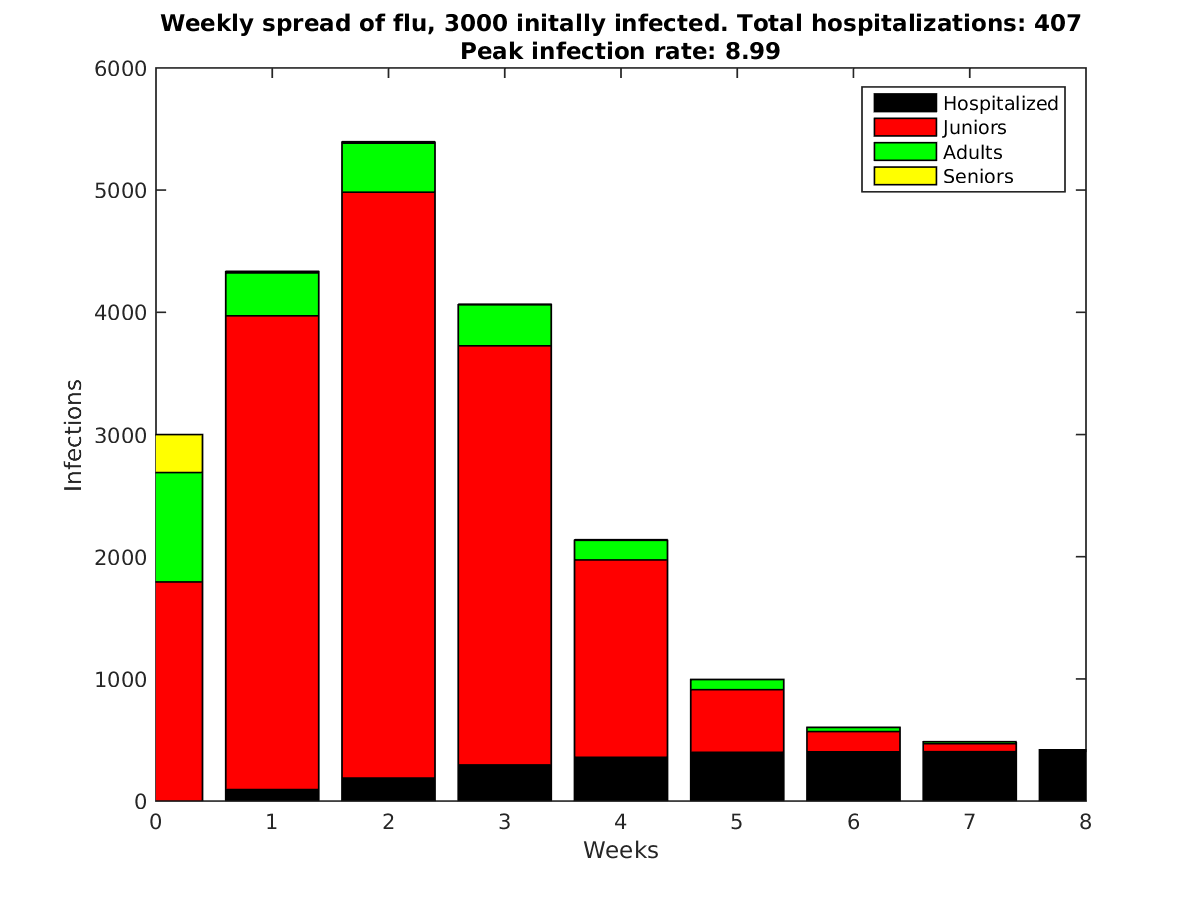
\includegraphics[width=\textwidth]{figures/Weekly-randvax.png}
		\caption{Random vaccination policy}
	\end{subfigure}\\
	\begin{subfigure}[b]{0.5\textwidth}
		\centering
		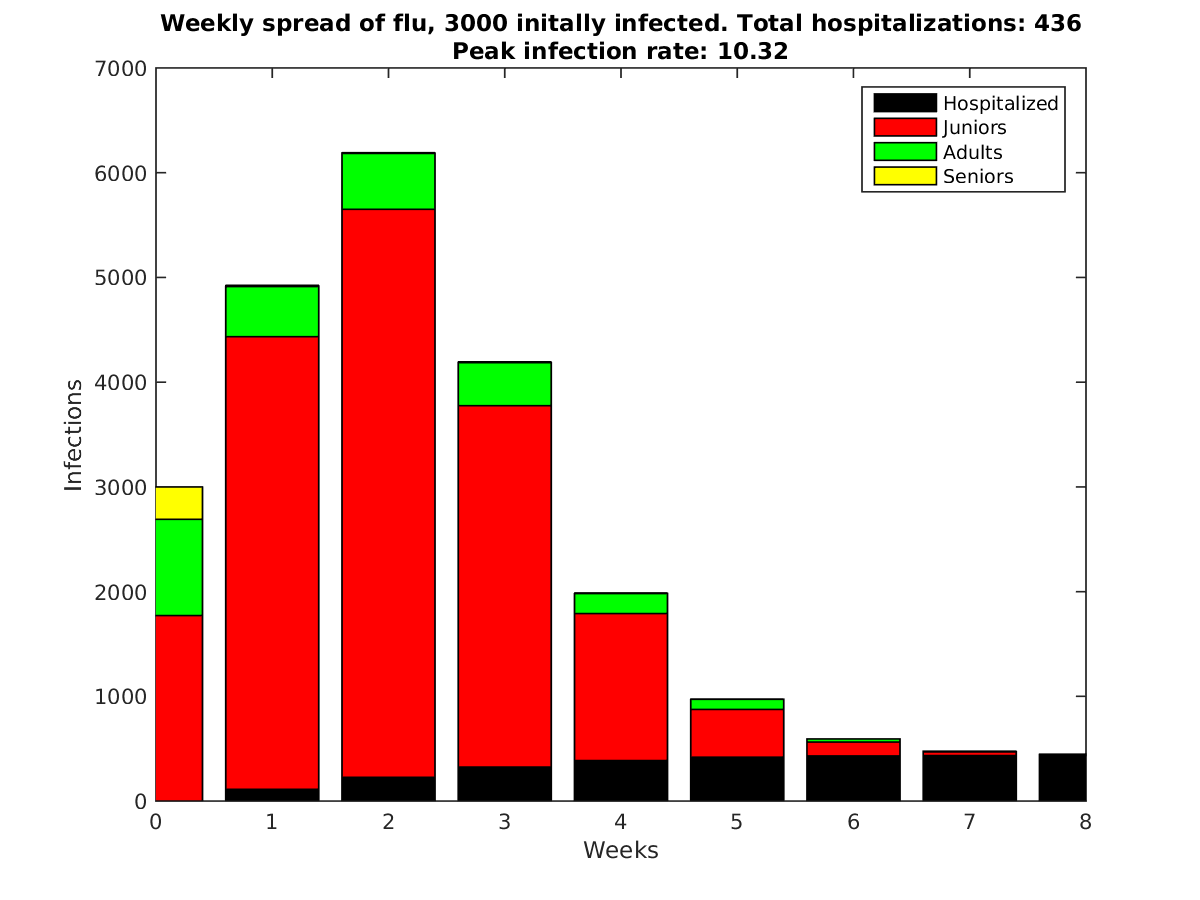
\includegraphics[width=\textwidth]{figures/Weekly-juniors.png}
		\caption{Prioritization of kids and teens}
	\end{subfigure}~
	\begin{subfigure}[b]{0.5\textwidth}
		\centering
		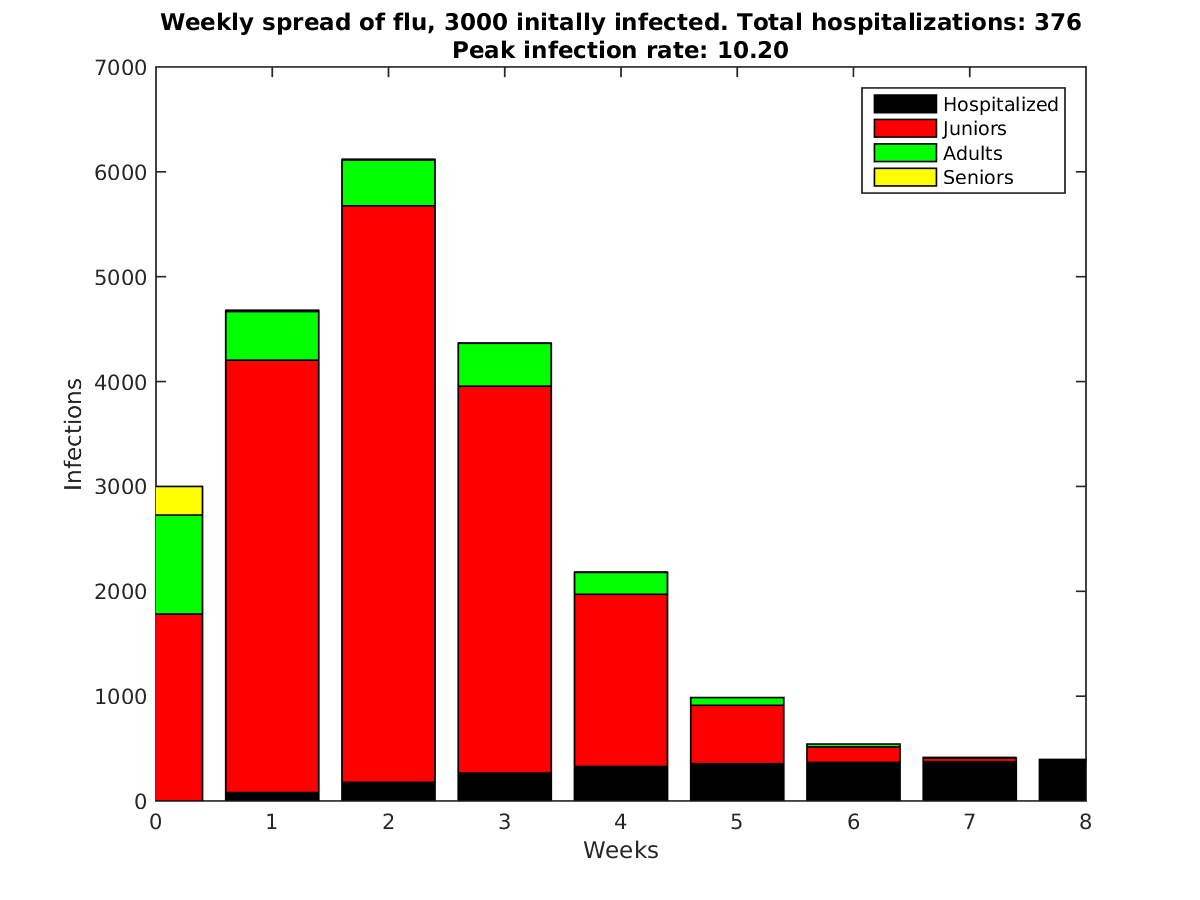
\includegraphics[width=\textwidth]{figures/Weekly-seniors.png}
		\caption{Prioritization of seniors}
	\end{subfigure}
	\caption{Model runs}
	\label{fig:modelout}
\end{figure}

Which unfortunately doesn't look promising.

\subsection{Analysis}
\par As we saw in Figure~\ref{fig:modelout}, vaccination policies don't actually impact the spread of the disease too much. Rather, it seems to be more helpful for damage control. We see from the 4 graphs in Figure~\ref{fig:modelout} the peak infection rate seems to stay near 10\% regardless of the vaccination policy. On the other hand, it seems to help for damage control because even though the infection rate stays the same, when we vaccinate more seniors, fewer people end up hospitalized than when we target more juniors. But surprisingly, the random vaccination policy consistently came out on top. This peaked our interest, so we ran many simulations comparing the three models. Figure~\ref{fig:10outs} shows the outputs side by side. We see that the random policy actually puts just about as many people in the hospital as the policy that targets seniors, while keeping the peak infection rate actually lower than all the policies.

\begin{figure}[h!]
\centering
\begin{subfigure}[b]{0.5\textwidth}
\centering
\begin{tabular}{rc|c}
& Peak infection (\%) & Total hospitalizations\\ \cline{2-3}
& 11.1  & 431\\
& 10.62 & 418\\
& 9.47  & 433\\
& 8.9   & 414\\
& 11.11 & 404\\
& 10.24 & 411\\
& 11.35 & 442\\
& 10.59 & 412\\
& 10.88 & 432\\
& 10    & 395\\ \hline
Mean & 10.426 & 419.2
\end{tabular}
\caption{Juniors first}
\end{subfigure}~
\begin{subfigure}[b]{0.5\textwidth}
\centering
\begin{tabular}{rc|c}
& Peak infection (\%) & Total hospitalizations\\ \cline{2-3}
& 10.45 & 389\\
& 10.65 & 376\\
& 10.25 & 419\\
& 10.86 & 388\\
& 10.1  & 384\\
& 11.05 & 373\\
& 9.97  & 377\\
& 9.57  & 383\\
& 10.14 & 363\\
& 9.91  & 367\\ \hline
Mean & 10.295 & 381.9
\end{tabular}
\caption{Seniors first}
\end{subfigure}\\
\begin{subfigure}[b]{0.5\textwidth}
\centering
\begin{tabular}{rc|c}
& Peak infection (\%) & Total hospitalizations\\ \cline{2-3}
& 9.5   & 378\\
& 9.99  & 393\\
& 10.02 & 373\\
& 9.28  & 370\\
& 9.72  & 386\\
& 9.68  & 369\\
& 10.25 & 423\\
& 10.36 & 415\\
& 9.11  & 370\\
& 9.96  & 352\\ \hline
Mean & 9.787 & 382.9
\end{tabular}
\caption{Indiscriminate vaccinations}
\end{subfigure}
\caption{Comparison of 10 runs for different vaccination policies}
\label{fig:10outs}
\end{figure}


\begin{thebibliography}{9}
\bibitem{areconnect}
	\url{http://ithaca.areaconnect.com/statistics.htm}
\bibitem{CIC-stats}
	\url{http://www.cdc.gov/h1n1flu/surveillanceqa.htm}
\bibitem{CIC-qa}
	\url{http://www.cdc.gov/h1n1flu/qa.htm}
\bibitem{walph}
	Wolfram Research Inc.,
	\emph{WolframAlpha},
	Retrieved September 26, 2015
	\url{http://www.wolframalpha.com/input/?i=\%E2\%88\%AB+e\^\%28-a+x\^2+\%2B+b+x\%29+dx}
	\url{http://www.wolframalpha.com/input/?i=ds\%2Fdt+\%3D+r+s+\%28K+-+s+-+a+t\%29}
\bibitem{census}
	http://quickfacts.census.gov/qfd/states/36/3638077.html
\bibitem{cornellpop}
	https://www.cornell.edu/about/facts.cfm
\end{thebibliography}


\end{document}
